\documentclass[tikz,border=5]{standalone}
\usetikzlibrary{decorations.pathmorphing}
\usepackage[detect-all]{siunitx}

\tikzset{
   ragged border/.style={ decoration={random steps, segment length=1mm, amplitude=0.5mm},
           decorate,
   }
}

\def\hh{0000}
\pgfmathsetmacro{\hhh}{0.8*\hh}
\pgfmathsetmacro{\hout}{min(0.3, \hh)}

\begin{document}
  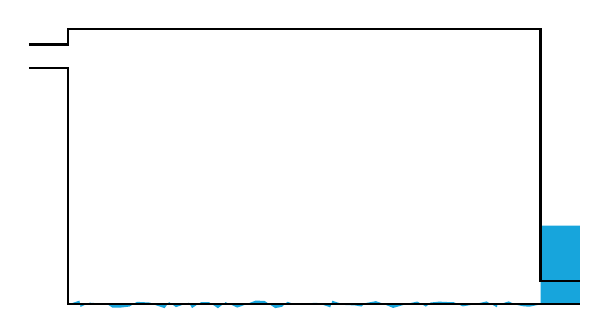
\begin{tikzpicture}
  \fill[black!10!cyan]
        decorate[ragged border]{
        (0,\hh) -- (6,\hh)
        }
        -- (6,\hout) -- (6.5,\hout) -- (6.5,0.0) -- (6,0.0) --(6,0) -- (0,0) -- cycle;
  %\fill[black!10!cyan] (-0.5,3) -- (0,3) to[in=90,out=0](0.7,\hhh)-- (1.0,\hhh)
  %                to[out=90,in=0] (0,3.3) -- (-0.5,3.3) -- cycle;
  \draw[thick] (-0.5,3) -- (0,3) -- (0,0) -- (6,0) -- (6,0.0) -- (6.5,0.0);
  \draw[thick] (-0.5,3.3) -- (0,3.3) -- (0,3.5) -- (6,3.5) -- (6,0.3) -- (6.5,0.3);
  %\draw[|-|] (-0.2,0) --
  %      node[fill=white,font=\footnotesize,inner ysep=2pt,inner
  %              xsep=0, anchor=east]{}(-0.2,\hh);
  %\draw[stealth-] (-0.5,2.75) -- (-1,2.75)
  %          node[anchor=east,font=\footnotesize,align=right]{};
  %\draw[-stealth] (6.5,0.15) -- (7.2,0.15)
  %          node[anchor=west,font=\footnotesize]{};
  \node[anchor=north,font=\footnotesize] at (3,3) {};
  \node[anchor=north,font=\footnotesize] at (3,2) {};
  \node[anchor=north,font=\footnotesize] at (3,1) {};
\end{tikzpicture}%
\end{document}